% !TEX root = ../../main.tex

\subsection{Crystalinity of leached samples}\label{def:xrd}

\begin{wrapfigure}[15]{r}{0.3\textwidth}
    \centering
    \captionsetup{format=plain}
    \fbox{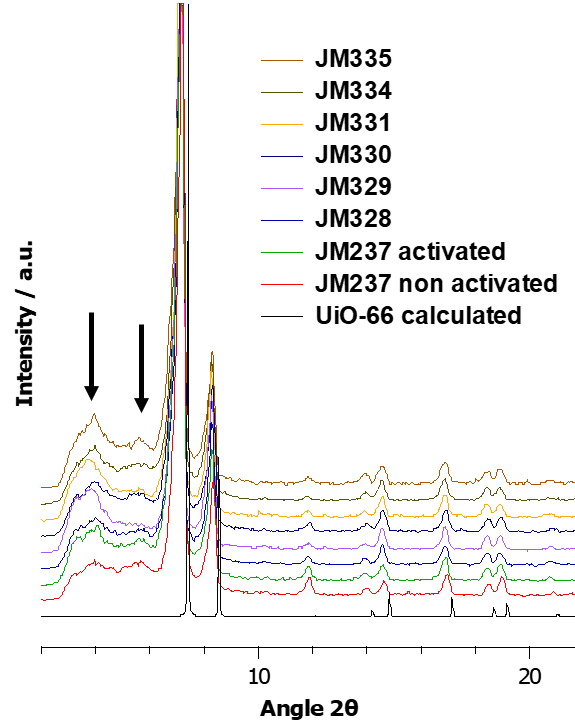
\includegraphics[width=0.28\textwidth]{xrd/xrd-h2o-peaks}}
    \caption{Diffuse scattering peaks in the \ce{H2O} leached 
    samples.}%
    \label{def:fgr:xrd-defects}
\end{wrapfigure}

The crystalinity of the leached samples is verified through 
XRD. The results in \autoref{appx:def:xrd} confirm that all 
resulting materials retain the same peaks in their powder
diffraction patterns.

A closer look at the low angle scattering (\autoref{def:fgr:xrd-defects})
reveals the appearance of diffuse peaks, corresponding to forbidden
reflections of the (\textbf{reo}) phase. They confirm that the 
leached samples begin to exhibit phase coexistence of 
the original UiO-66(Zr) unit cell and the missing cluster
(\textbf{reo}) net. These peaks have the highest intensity in 
the TFA treated materials, suggesting that it has the highest 
capability of introducing missing cluster defects.